%----------------------------------------------------------------------------------------
%    PACKAGES AND THEMES
%----------------------------------------------------------------------------------------

\documentclass[aspectratio=169,xcolor=dvipsnames]{beamer}
\usetheme{SimpleDarkBlue}

\usepackage{hyperref}
\usepackage{graphicx} % Allows including images
\usepackage{booktabs} % Allows the use of \toprule, \midrule and \bottomrule in tables

%----------------------------------------------------------------------------------------
%    TITLE PAGE
%----------------------------------------------------------------------------------------

\title{Multi-core scheduling}
\subtitle{Performance Evaluation of Computer Systems and Networks project}

\author{Taulant Arapi (645308)\\Francesco Barcherini (645413)\\Antonio Ciociola (645324)}
\date{\today} % Date, can be changed to a custom date

%----------------------------------------------------------------------------------------
%    PRESENTATION SLIDES
%----------------------------------------------------------------------------------------

\begin{document}

\begin{frame}
    % Print the title page as the first slide
    \titlepage
\end{frame}

\begin{frame}{OMNeT++ Model}
    \begin{columns}[c] % The "c" option specifies centered vertical alignment while the "t" option is used for top vertical alignment

    \column{.45\textwidth} % Left column and width
    \begin{itemize}
        \item Process generator: exponential inter-arrival time and duration
        \item Scheduler: infinite FIFO queue or priority queue (FCFS/SJF)
        \item CPU: $N$ of them (4 or 12)
    \end{itemize}

    \column{.45\textwidth} % Right column and width
    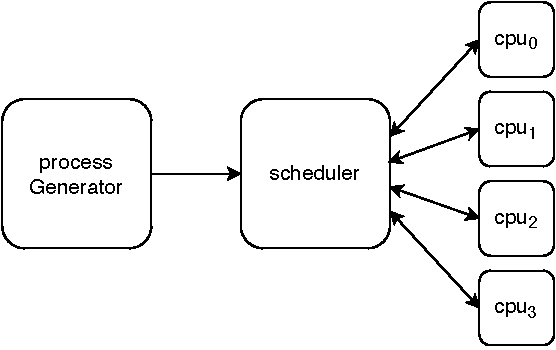
\includegraphics[width=\textwidth]{files/Computer.pdf} % oppure files/sim_schema.png
\end{columns}
    
\end{frame}

%------------------------------------------------

\begin{frame}{Stability / Validation / cazzo ne so}
    In this slide, some important text will be \alert{highlighted} because it's important. Please, don't abuse it.

    \begin{block}{Block}
        Sample text
    \end{block}

    \begin{alertblock}{Alertblock}
        Sample text in red box
    \end{alertblock}

    \begin{examples}
        Sample text in green box. The title of the block is ``Examples".
    \end{examples}
\end{frame}

%------------------------------------------------

\begin{frame}{Casi particolari?}
    \begin{columns}[c] % The "c" option specifies centered vertical alignment while the "t" option is used for top vertical alignment

        \column{.45\textwidth} % Left column and width
        \textbf{Heading}
        \begin{enumerate}
            \item Statement
            \item Explanation
            \item Example
        \end{enumerate}

        \column{.45\textwidth} % Right column and width
        Lorem ipsum dolor sit amet, consectetur adipiscing elit. Integer lectus nisl, ultricies in feugiat rutrum, porttitor sit amet augue. Aliquam ut tortor mauris. Sed volutpat ante purus, quis accumsan dolor.

    \end{columns}
\end{frame}

%------------------------------------------------
\section{Second Section}
%------------------------------------------------

\begin{frame}{Table}
    \begin{table}
        \begin{tabular}{l l l}
            \toprule
            \textbf{Treatments} & \textbf{Response 1} & \textbf{Response 2} \\
            \midrule
            Treatment 1         & 0.0003262           & 0.562               \\
            Treatment 2         & 0.0015681           & 0.910               \\
            Treatment 3         & 0.0009271           & 0.296               \\
            \bottomrule
        \end{tabular}
        \caption{Table caption}
    \end{table}
\end{frame}

%------------------------------------------------

\begin{frame}{Warm-up and Simulation Time}
    \begin{theorem}[Mass--energy equivalence]
        $E = mc^2$
    \end{theorem}
    This theorem gives us the exact values of the warm-up and simulation time.
\end{frame}

%------------------------------------------------

\begin{frame}{Statistiche statistiche}
    Uncomment the code on this slide to include your own image from the same directory as the template .TeX file.
    %\begin{figure}
    %\includegraphics[width=0.8\linewidth]{test}
    %\end{figure}
\end{frame}

%------------------------------------------------

\begin{frame}{First Come First Served}
    grafici molto bellini
\end{frame}

%------------------------------------------------

\begin{frame}{Shortest Job First}
\end{frame}

%------------------------------------------------

\begin{frame}{Conclusions}
    \centerline{\textbf{Vogliamo dedicarle una slide?}}
\end{frame}

%----------------------------------------------------------------------------------------

\end{document}
